\chapter{项目实现}
\section{实现概述与阅读口径}
在第四组报告的“Bug 修复及功能完善、商家功能、用户功能”基础上，本章扩展骑手、管理员、AI 与资产模块。以下实现说明来自当前仓库源码；界面图来自项目已保存的截图。对于文档与代码仍有差异的部分，报告在第五章集中列出，不把设计意图写成已经完成的行为。

仓库前端使用 Vue 3，但仅凭当前版本不能证明本组完成了某一次完整的 Vue 2 升级过程。因此，本报告重点说明现有架构与业务完善，不直接继承参考报告中的版本迁移经历或其特定故障记录。
\section{顾客端实现}
\subsection{首页与个人中心}
首页承担店铺发现和点餐入口功能，包括搜索、分类、推荐与店铺信息展示。顾客可从首页进入门店详情，查看商品和配送条件，再将商品加入购物车。个人中心集中提供资料、地址、收藏、消息及账号操作，避免把非交易设置分散在点餐链路中。
\begin{figure}[H]\centering
\begin{minipage}[t]{.46\linewidth}\centering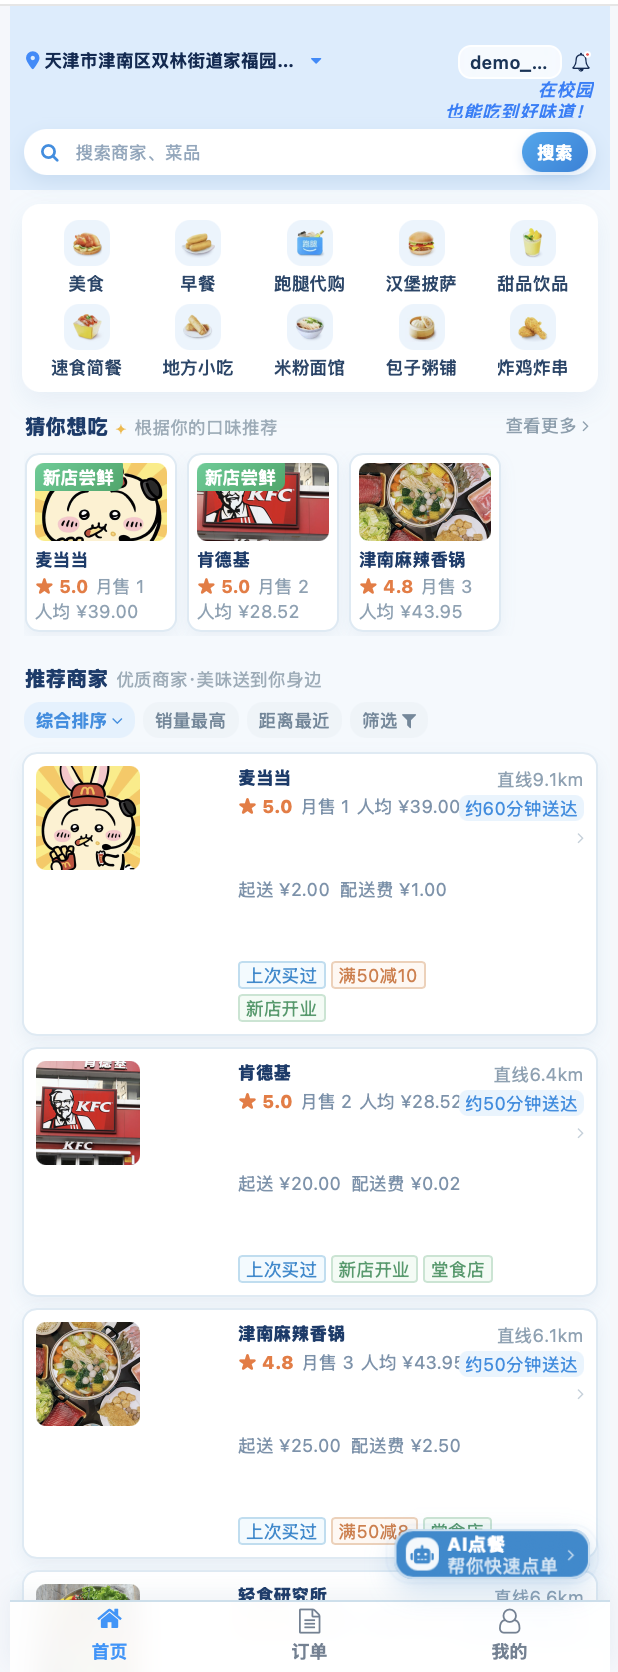
\includegraphics[height=.55\textheight,width=\linewidth,keepaspectratio]{figures/report/home.png}\par\small 首页与店铺发现\end{minipage}\hfill
\begin{minipage}[t]{.46\linewidth}\centering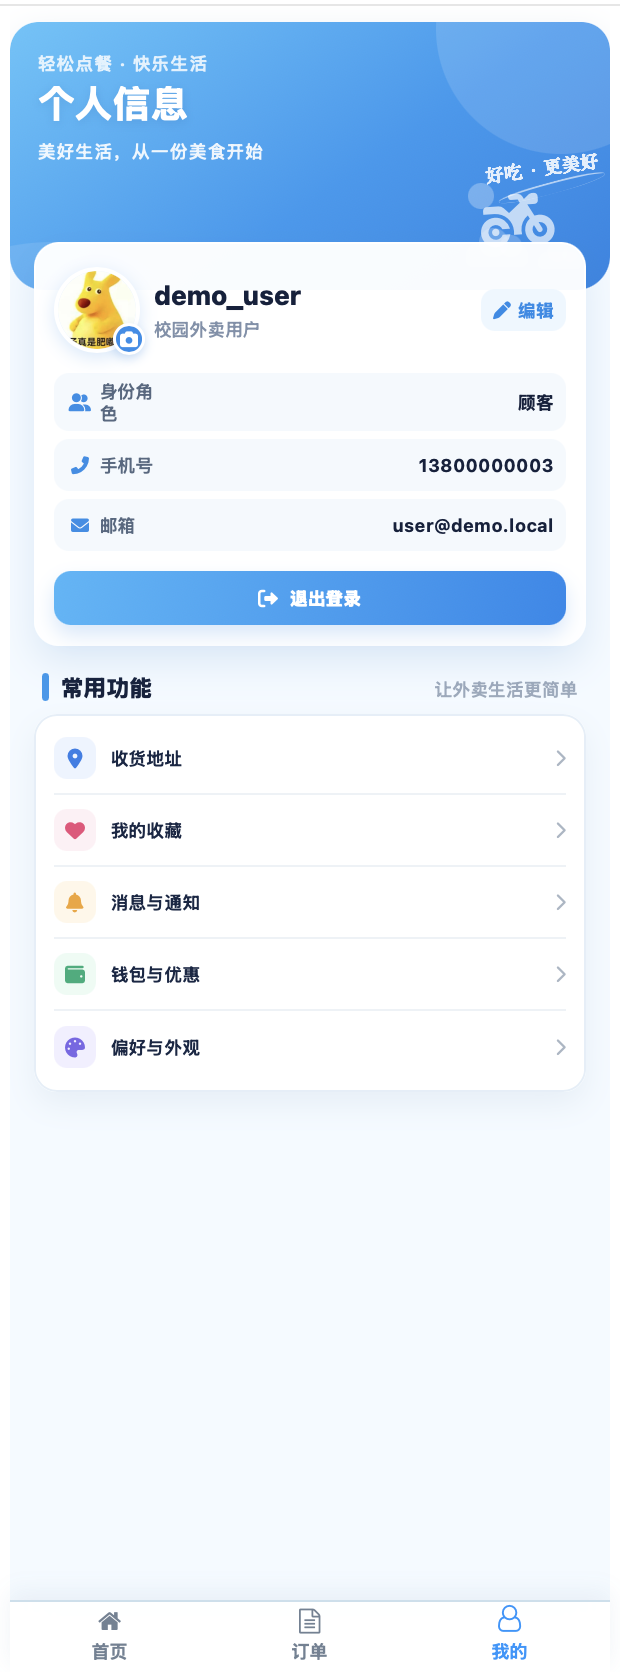
\includegraphics[height=.55\textheight,width=\linewidth,keepaspectratio]{figures/report/customer.png}\par\small 顾客个人中心\end{minipage}
\caption{顾客端已有界面截图（演示数据）}\end{figure}
\subsection{购物车与选中商品结算}
当前提交服务先读取当前用户在指定商家的购物车，再根据选中商品集合筛选提交项。若选中商品已经变化，不能静默忽略后继续创建与用户预期不同的订单，而应提示重新选择。订单成功写入后，只清理已经提交的条目。

购物车数量和限购在后端重新校验，不能依赖前端加减按钮的最大值。当前服务还限制单笔订单的商品种类，并对同一商品的数量进行合并校验，避免通过拆成多行绕过限购规则。
\subsection{订单创建与数据快照}
\code{OrderSubmissionService} 按“店铺与履约方式—用户身份—幂等键—地址—购物车—报价—库存—订单明细”的顺序组织下单。店铺必须满足审核与营业条件；外送地址必须存在且属于本人；商品数量和价格应有效。

库存预占使用带条件的数据库更新，更新失败表示库存不足或商品不可售。下单服务在事务中保存订单及商品明细快照，复制联系人、电话和地址，并记录订单创建历史。这样，即使后续修改商品或个人地址，历史订单仍具有独立的业务含义。

请求携带可用幂等键时，服务先查询同一用户是否已经创建对应订单。该机制为重复提交提供保护，但仍需通过并发和异常重试测试核验边界，不能仅凭存在幂等字段就宣称所有重复请求均已覆盖。
\subsection{服务端计价与支付边界}
\code{OrderPricingService} 使用 \code{BigDecimal} 计算金额，根据真实商品价格和数量计算小计，校验外送起送价，再处理商家满减、有效会员折扣及配送费。到店自取不收取外送费用，也不要求按外送规则提供地址。

\code{OrderSettlementService} 进一步校验优惠券归属和门槛、积分余额与抵扣上限，执行钱包或模拟支付。当前积分抵扣要求为 100 的整数倍，且不能超过券后应付金额的 20\%。优惠券扣减、积分扣减、钱包扣减和订单支付记录应在业务事务中保持一致。

以商品小计 40 元、商家满减 5 元、有效会员 95\% 折扣、配送费 3 元、优惠券 5 元、抵扣 500 积分为例，按当前源码规则可计算为：
\begin{align*}
\text{提交金额}&=(40-5)\times0.95+3=36.25\text{ 元},\\
\text{券后金额}&=36.25-5=31.25\text{ 元},\\
\text{积分上限折算金额}&=31.25\times20\%=6.25\text{ 元},\\
\text{实际应付}&=31.25-5=26.25\text{ 元}.
\end{align*}
以上是规则演算示例，并非实际订单截图或压测数据。是否满足优惠券门槛、是否拥有足额积分等前置条件仍需同时成立。该例也说明为什么优惠顺序必须写清：若先后次序不同，同一组参数就可能得到不同金额。

后端对 \code{alipay} 和 \code{wechat} 真实支付标记进行拒绝，明确提示尚未接入服务端回调；模拟支付仅在课程演示配置开启时允许。页面展示支付品牌不能被表述为已经实现真实支付能力。
\section{商家端实现}
商家端将商家身份与具体店铺经营资源关联，提供店铺资料、商品和订单入口。商品维护需要同时考虑价格、库存、分类、上下架与限购，并通过服务端校验店铺归属。

履约服务在商家接单时将待接单订单推进到后续阶段；拒单时执行取消和结算回退；出餐时根据外送或自取分流。外送生成配送任务，自取进入待取餐阶段，不生成虚假的骑手任务。评价回复和经营展示建立在同一店铺边界之内。

\section{骑手端实现}
骑手端根据审核和在线状态决定是否允许领取任务。任务领取并非“查询为空后直接写入”，而是调用数据库原子更新，并检查受影响行数。只有任务仍满足可领取条件时才能绑定骑手，其他竞争请求得到冲突提示。

当前实现把“到店”作为独立配送任务状态。骑手需先到店再取餐，取餐后同步推进订单至配送中，送达后通知顾客确认。每一步都检查任务归属，避免通过修改任务编号操作他人任务。

异常上报与管理员处置形成另一条重要链路。异常不应只停留在骑手页面的文字说明中，还需关联订单与任务，为恢复或改派提供依据。导航服务失败时保留文本地址，避免地图故障阻断履约。
\begin{figure}[H]\centering
\begin{minipage}[t]{.47\linewidth}\centering
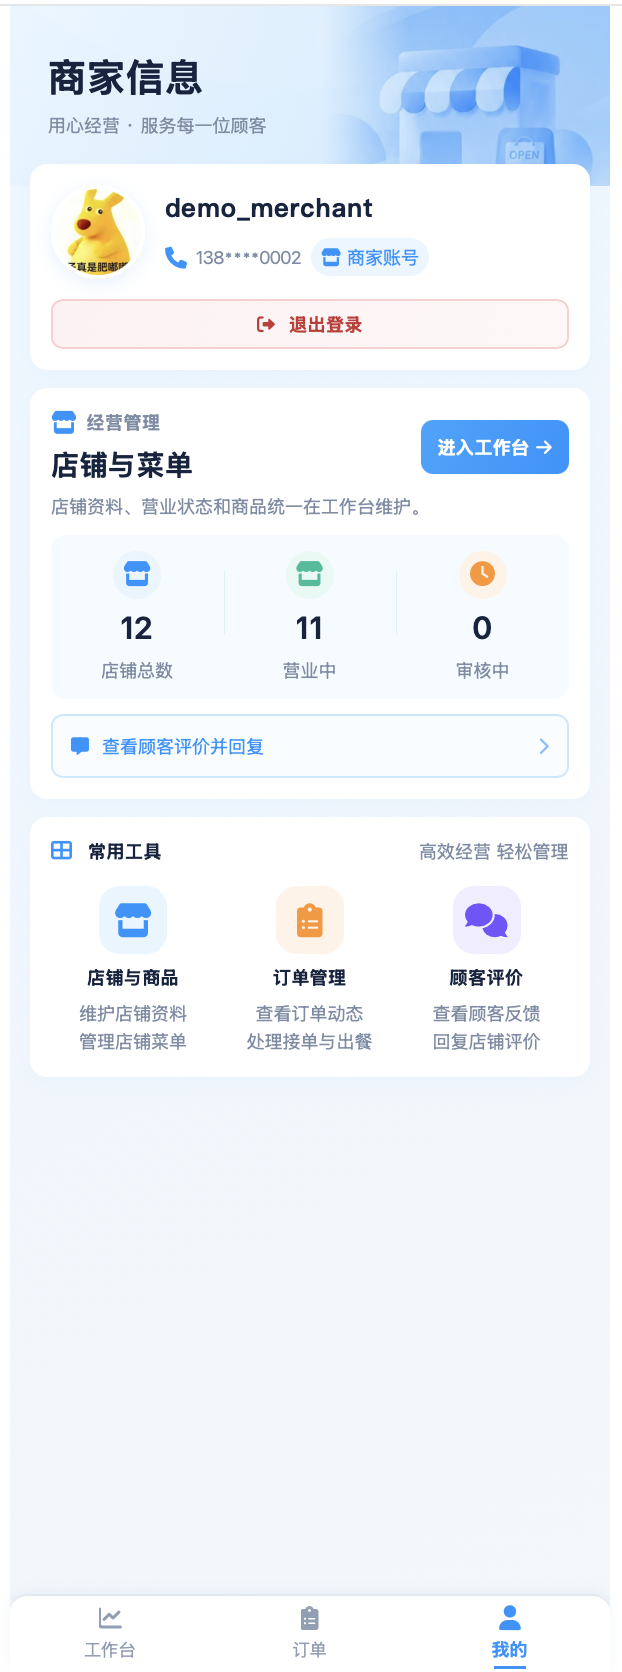
\includegraphics[height=.54\textheight,width=\linewidth,keepaspectratio]{figures/report/merchant.png}\par\small 商家端：店铺、商品与经营入口
\end{minipage}\hfill
\begin{minipage}[t]{.47\linewidth}\centering
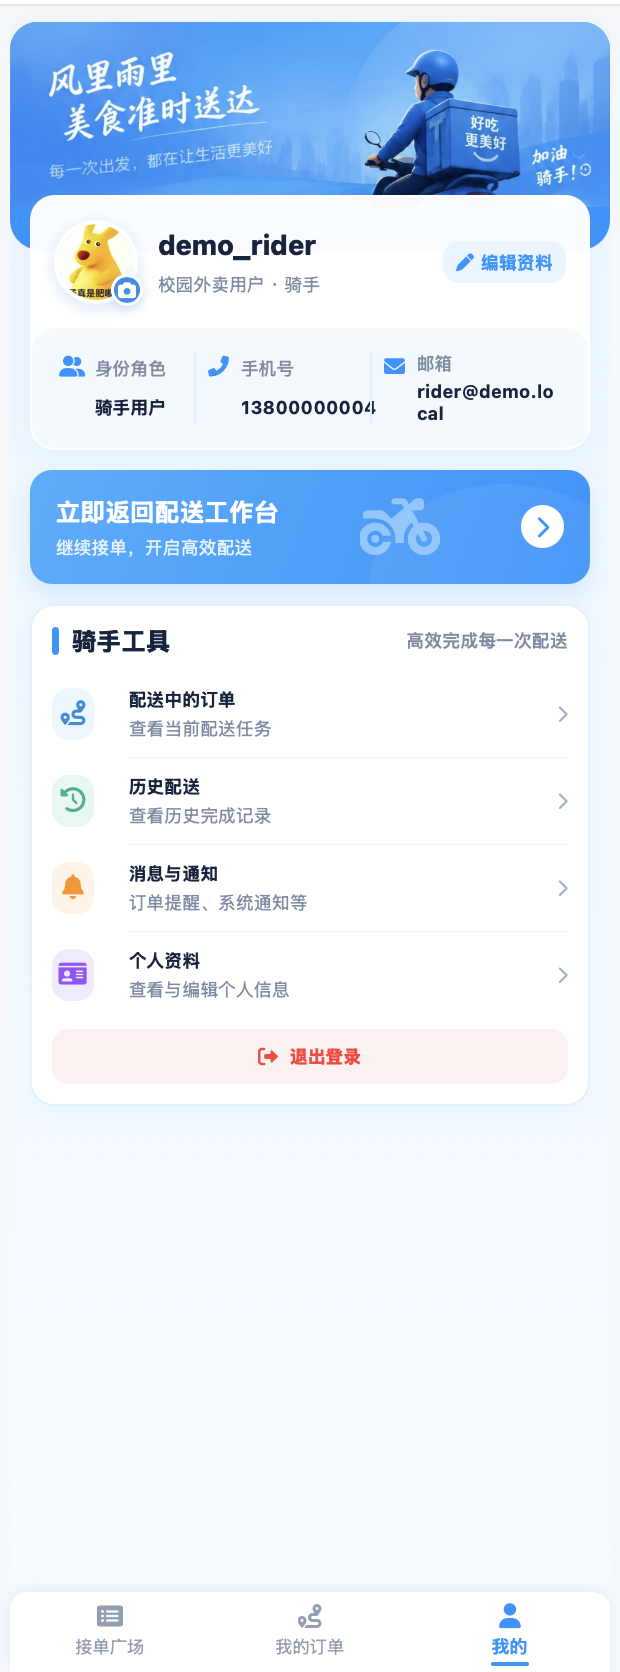
\includegraphics[height=.54\textheight,width=\linewidth,keepaspectratio]{figures/report/rider.png}\par\small 骑手端：任务与配送入口
\end{minipage}
\caption{商家端与骑手端界面（项目已有截图）}\end{figure}
\section{管理员端实现}
管理员端提供准入审核、账号管理和平台统计入口，承担跨角色的治理职责。审核后的权限变化应由后端重新识别，不能仅通过前端显示审核结果完成授权。平台数据看板应使用统一日期范围和订单口径，并在无数据时显示合理空状态。

管理员操作的影响往往跨越多个模块。例如停用账号可能影响令牌会话，配送异常处置可能影响骑手当前任务和订单状态。因此，管理功能的测试应覆盖后续行为，而不仅是检查审核按钮返回成功。
\begin{figure}[H]\centering
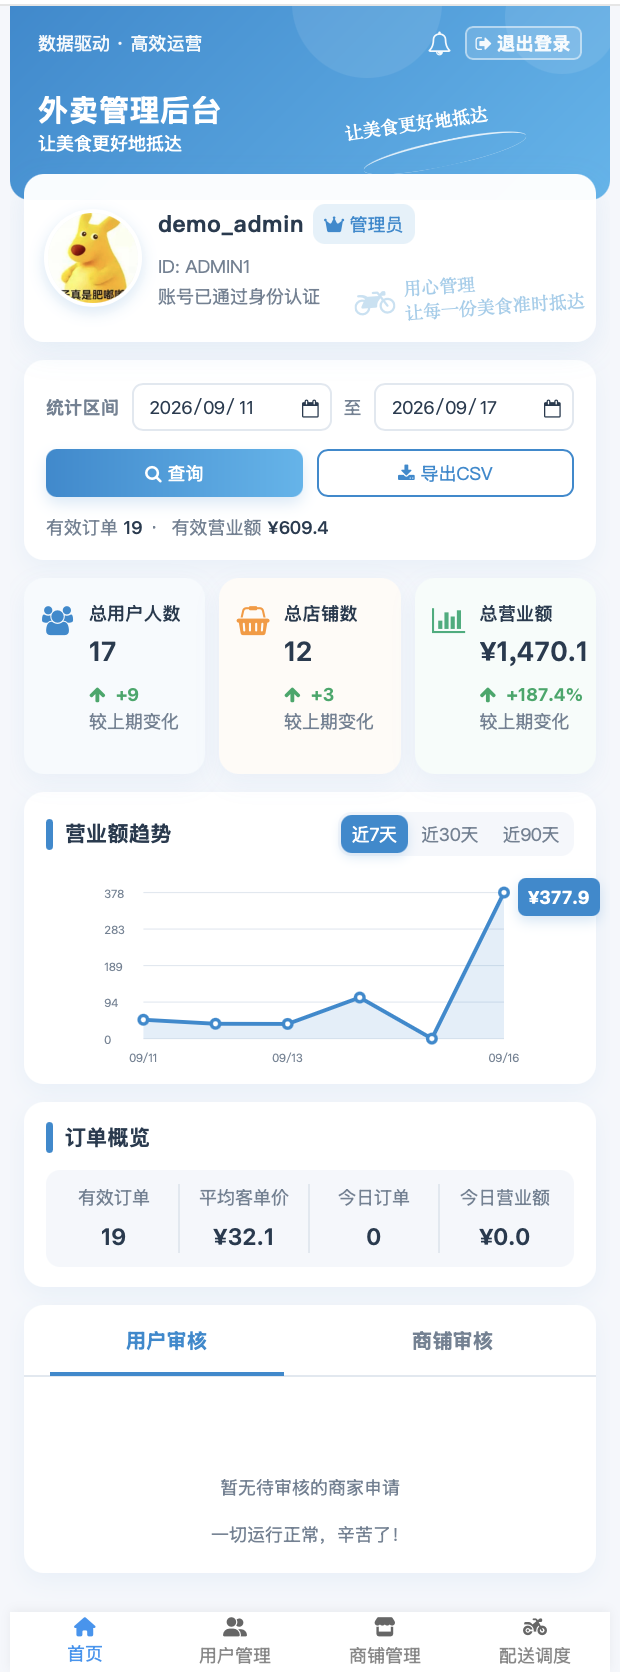
\includegraphics[height=.58\textheight,width=.65\linewidth,keepaspectratio]{figures/report/admin.png}
\caption{管理员平台统计及管理入口（已有截图，数值为演示数据）}\end{figure}
\section{AI 客服与智能点餐实现}
\subsection{意图分流与结构化响应}
\code{StructuredAssistantServiceImpl} 对输入执行本地意图判定，将问题分为推荐、规则、订单和一般对话。规则类请求可以本地答复，推荐请求交给推荐服务；订单和一般对话则进入对话服务。响应同时携带意图、文本、会话、候选商品、是否需要确认以及处理耗时。

这种结构让前端能够显示可点击商品候选，而不是从自然语言中猜测商品名称。推荐服务验证预算与数量，按用户是否授权使用偏好决定是否读取个人偏好，再交给适配器检索候选。当前存在基于规则的推荐实现，因此“AI 点餐”并不意味着每一步都必须请求大模型。
\subsection{真实业务数据与授权}
\code{AiChatServiceImpl} 从认证上下文确定用户，不信任请求中的用户编号。订单上下文只纳入归属当前用户的订单，具体订单不可见时返回无可查询结果，不能把他人数据交给模型后再期待模型自行保密。

外部对话请求在模型输入中加入平台规则和经过筛选的数据库上下文，并明确将数据库内容作为数据处理。对话历史受会话归属检查约束，外部网络调用结束后再保存历史。日志对消息正文进行隐藏处理，减少记录敏感内容的机会。
\subsection{失败降级与调用次数}
配置了有效外部服务凭证时，对话服务尝试调用模型；调用失败或结果不可用时使用本地帮助。客户端具有总体超时与错误重试逻辑，源码默认重试参数为 3。这里的“3 次重试”与答辩中讨论的“一个问题调用 3 次模型”是两个概念：初始尝试加 3 次重试，理论上最多可能产生 4 次尝试，实际次数还受总超时限制。

当前代码不能支持“所有问题固定调用三次”的描述。答辩中的三次调用问题应作为所讨论方案的效率分析，与当前意图分流、实际请求次数及失败重试分别说明。系统虽然包含熔断工具类，但仍需要核对每个外部调用是否真正接入，不能以工具类存在代替全链路保护完成的证据。
\subsection{图片与语音入口}
仓库提供图片识菜和语音订单草稿接口。媒体入口先进行格式、大小等校验，再通过外部识别适配器处理。识别结果应转换为候选或草稿，交由用户核对；不能直接扣库存、付款或修改资产。

这些功能受外部服务配置、网络和识别质量影响。课程演示应预先说明启用条件，并准备文本输入与普通搜索作为替代路径。报告不把接口存在等同于真实外部服务已完成全部验证。
\section{通知、资产与部署}
订单、配送与审核的重要变化通过通知服务传递，消息持久化与即时展示各有作用：即时推送用于及时提醒，历史列表用于用户重新进入页面后追溯。通知失败不能让已经提交的业务事实消失，用户也应能够重新查询权威状态。

资产服务集中维护余额、积分和优惠券，支付、取消、完成订单各使用明确的业务入口。部署方面，仓库提供 Docker Compose、初始化脚本和部署说明，便于在统一演示环境中还原四端联调。配置与源码分离，外部服务密钥由环境变量或服务端配置提供。
